\documentclass[10pt,a4paper]{article}
\usepackage[utf8]{inputenc}
\usepackage[polish]{babel}
\usepackage[T1]{fontenc}
\usepackage{amsmath}
\usepackage{amsfonts}
\usepackage{amssymb}
\usepackage{graphicx}
\nonstopmode

\title{Flow-Shop Scheduling\\Laboratorium Optymalizacji Kombinatorycznej}

\author{Szymon Gramza\\
  szymon.gramza@student.put.poznan.pl
\and
  Maciej Sobkowski\\
  maciej.sobkowski@student.put.poznan.pl
\and
  Prowadzący: Marcin Radom
}

\begin{document}
\maketitle
\section{Wprowadzenie}
\subsection{Opis problemu}
Problem Flow-Shop jest problemem optymalizacji kobminatorycznej, który polega na
szeregowaniu zadań przy wykorzystaniu ustalonej liczby maszyn. Każde zadanie
składa się z listy operacji, które muszą zostać wykonane w określonej kolejności
na określonej maszynie, a każdą operację cechuje czas wykonywania. Zadania
pojawiają się w różnych momentach pracy systemu, a maszyny na których są
wykonywane posiadają wymuszone przestoje.  Do rozwiązania powyższego problemu
wykorzystaliśmy zainspirowaną zachowaniem się mrówek poszukujących pożywienia
metaheurystykę ACO\@. Algorytm mrówkowy będziemy porównywać z rozwiązaniem
uzyskanym za pomocą algorytmów losowego oraz rozwiązaniem optymalnym obliczonym
za pomocą wzoru: 
\[ opt = \frac{\text{suma\ czasów\ wszystkich
operacji}}{\text{liczba\ maszyn}} \]

\subsection{Program testujący}
\subsubsection{Opis}
Aplikacja została napisana w języku C i wykorzystuje biblioteki dostępne w
systemach z rodziny GNU/Linux. 
\subsubsection{Kompilacja}
Kompilacja została zautomatyzowana przy pomocy programu GNU Make. Aby
skompilować program należy z poziomu konsoli wydać polecenie \textit{make}.
Prawidłowe zakończenie procesu kompilacji zostanie zasygnalizowane komunikatem
\textit{Zakończono linkowanie!}.
\subsubsection{Uruchomienie}
Praca aplikacji jest sterowana przez przełączniki powszechnie stosowane w
oprogramowaniu linuksowym.  Przykładowe wywołanie \textit{scheduler -i
inst\_name -o file\_name.csv} uruchomi program dla instancji zapisanej w pliku
inst\_name i wykona algorytm ACO oraz losowy. Wynik szeregowania zostanie
zwrócony do pliku o nazwie file\_name.csv.  Dodatkowo, aby uruchomić program
generujący instancje należy użyć polecenia \./generator.\\ Przykładowe wywołanie
\textit{./generator -i input\_name -o inst\_name } spowoduje wygenerowanie pliku
instancji inst\_name przyjmując parametry zawarte w pliku input\_name zgodnie ze
schematem, że każda linia składa się z 5 liczb całkowitych, które odpowiednio
charakteryzują: liczbę zadań, początek i koniec przedziału czasu wykonania
operacji, początek i koniec przedziału czasu gotowości zadania.\\ Generator
losuje czasy wykonania operacji i czasy gotowości dla zdefiniowanej liczby
zadań.

\section{Algorytm Ant Colony Optimization}
\subsection{Opis algorytmu}
Zastosowana przez nas metaheurystyka - Ant Colony Optimization - opiera się na
naturalnym zachowaniu kolonii mrówek poszukujących pożywienia. Algorytm korzysta
ze struktur utrzymujących informację o drodze od źródła do celu, przebytej przez
każdą mrówkę danego pokolenia. Algorytm został zaprojektowany do problemów
znajdowania ścieżki w grafie o najmniejszym koszcie (problem TSP).
Przystosowanie algorytmu do problemu szeregowania zadań sprowadza się w naszym
przypadku do przedstawienia operacji danej instancji w postaci grafu, którego
przykład umieszczono poniżej:\\
\begin{center}
    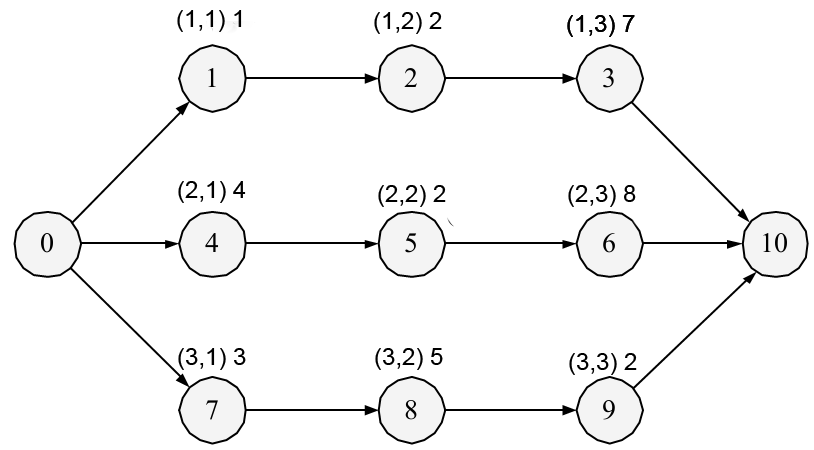
\includegraphics [scale=0.4]{./figures/pic01.png}\\
\end{center}
Każdemu wierzchołkowi grafu przyporządkowana jest jedna operacja, każda operacja zaś posiada informacje o maszynie i numerze zadania.
Zależności pomiędzy kolejnością wykonania operacji reprezentują łuki między nimi, ponadto graf posiado dwa dodatkowe wierzchołki - początkowy i końcowy - które pozwalają przypisać pierwszej i ostatniej operacji feromon. Dzięki takiej reprezentacji problemu możemy korzystać z wzorów przeznaczonych dla algorytmu TSP z drobnymi modyfikacjami.

Informacje o ilości feromonów utrzymywane są w macierzy NxN (N - liczba
operacji). 
Rozwiązaniem generowanym przez mrówkę jest łańcuch wszystkich wierzchołków zachowujący zależnosci między operacjami w zadaniu.
(sortowanie topologiczne) Przykładowy łańcuch: [0 1 4 2 7 5 8 3 6 9 10].

Przed uruchomieniam właściwego algorytmu, początkowa ilość feromonu na każdej ścieżce przyjmuje bardzo małą wartość, w naszej implementacji przyjęliśmy $ \tau_0 = 0.001 $ 

Każda mrówka wybierając drogę stosuję regułę zmiany stanu (State Transition Rule), którą obrazuje poniższy wzór:\\
%wzory do wklejenia
\begin{equation}
 s = \left\{ 
  \begin{array}{l l}
    arg\ max_{u \in J(r)} \{ [\tau (r,u)] \cdot [\eta (r,u)^\beta] \} , & \quad \text{jeśli $q\leq q_0$}\\
    S, & \quad \text{w przeciwnym razie}
  \end{array} \right.
\end{equation} \\
gdzie:
\begin{itemize}
  \item a  
  \item b
  \item c
\end{itemize}



dokonuje losowo, a wpływ pozostawionych feromonów uzyskaliśmy stosując
psuedo-ruletkę, która zwiększa prawdopodobieństwo wylosowania danej drogi
przydzielając “pasmo dostępności” danej drogi w losowanym zakresie w zależności
od aktualnej wartości feromonu.  W rozwiązaniu przyjęto także element parowania
pozostawionych feromonów, którą można wygodnie regulować za pomocą współczyniika
parowania.

Poszukiwanie rozwiązania opiera się na pętli z warunkiem wykonania wszystkich
zleceń, która wykonuje następujące kroki:
\begin{enumerate}
    \item dla każdej z maszyn: jeżeli maszyna jest bezczynna to na podstawie
      tablicy iteratorów znajdź zadanie przeznaczone dla tej maszyny (i zapisz
      czas jego rozpoczęcia) lub pozostań w stanie bezczynności,
    \item znajdź czas zadania, które kończy się najwcześniej i zapisz w zmiennej
      $t$,
    \item wykonaj $T += t$ i dla każdego aktualnie przetwarzanego zadania
      zmniejsz pozostały czas wykonania o $t$,
    \item jeżeli istnieje zadanie o pozostałym czasie wykonania równym 0, to
      usuń je z maszyny i przesuń iterator zlecenia o 1 w prawo.
\end{enumerate}

Po zakończeniu powyższej pętli długość uszeregowania znajduje się w zmiennej
$T$. 




\begin{equation}
 P(r,s) = \left\{ 
  \begin{array}{l l}
    \frac{[\tau (r,s)] \cdot [\eta (r,s)^\beta]}{\sum_{u \in J(r)} {[\tau (r,u)]
    \cdot [\eta (r,u)^\beta]}},
    & \quad \text{jeśli }s \in J(r)\\
     0, & \quad \text{w przeciwnym razie}
  \end{array} \right.
\end{equation}


\end{document}
